\documentclass[a4paper, 12pt]{article}
\usepackage[utf8]{inputenc}
\usepackage[left=3cm, top=3cm, right=2cm, bottom=2cm]{geometry}%ajusta as margens
\usepackage{setspace}
\setlength{\parindent}{1.25cm}%Altera o parágrafo
\usepackage{graphicx}
\usepackage[portuguese]{babel} 
\begin{document}

\begin{center}
    \large
    \textbf{Faculdade de Tecnologia Baixada Santista Rubens Lara\\}
    \textbf{Curso Superior de Tecnologia em Ciência de Dados}
    \vspace{6.5cm}\\
    Anderson Portes do Nascimento\\Breno Henrique Rey Lorenzo\\Kaylane Chavier Costa\\
    \vspace{6cm}
    \textbf{Determinante}
    \\
    \vspace{6cm}
    Santos, SP\\
    2022
\end{center}

\newpage
    \onehalfspacing
    \section{CÓDIGO PARA CALCULAR O DETERMINANTE}
    
    \par A partir da função "main", é pedido que o usuário digite o tamanho da matriz. Esse valor passado como paramtro à função "generateMatriz", que gera uma matriz quadrada de acordo com o número inserido. Por exemplo, se a matriz for 3x3, serão gerados 9 elementos. Se a matriz for 4x4, serão gerados 16 elementos e assim sucessivamente. OBS: A matriz é gerada com numeros sequenciais 
    Ainda dentro da função "main", será exibido o determinante da matriz gerada anteriormente. O determinante é calculado através da função "det". Primeiramente, a função det chama a função checkIsSquare, que verifica se a matriz é quadrada. Caso não seja, é lançado um erro ao  usuário exibindo a mensagem "a matriz não é quadrada". Caso seja quadrada, verifica-se se a matriz tem dimensão 2x2. Se for uma 2x2, o código é direcionado para calcular o determinante, multiplicando, primeiramente, os elementos da diagonal principal e, em seguida, os elementos da diagonal secundária, subtraindo os resultados no final.
    Em casos de matrizes  maiores que 2x2, a função det utilizara da função getDetSingleElement que calculará o determinante dos cofatorores de uma matriz. Nela, para calcular o determinante do cofator, o programa utiliza da função anteriormente execuatada "det", ou seja, é possível perceber a existência da recursividade entre essas duas funções, onde a computação se encerra quando o determinante do cofator for calculado a partir de uma matriz 2x2. Ao final dentro da função det é  gerado um vetor contendo os determinastes dos  cofatores e após isso é todos  os elementos são somados usando a função "sum" nativa do haskell retoranando o valor final do determinante da  matriz gerada.

    \begin{figure}[!ht]
        \centering
        \caption{Código para calcular o determinante}
        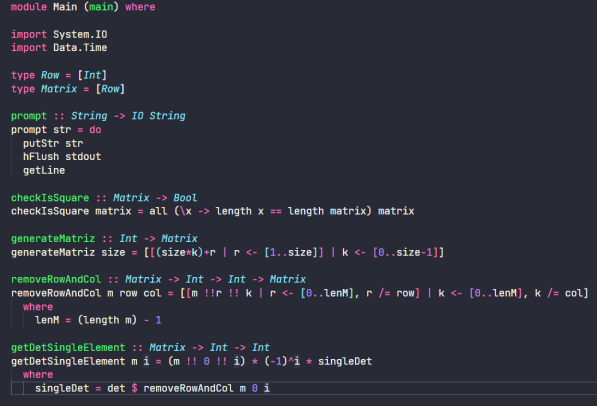
\includegraphics[scale=0.5]{codigo1.png} \\
        {\footnotesize Fonte: Elaborada pelo autor.}
        \label{fig:my_label}
    \end{figure}

    \begin{figure}[!ht]
        \centering
        \caption{Código para calcular o determinante}
        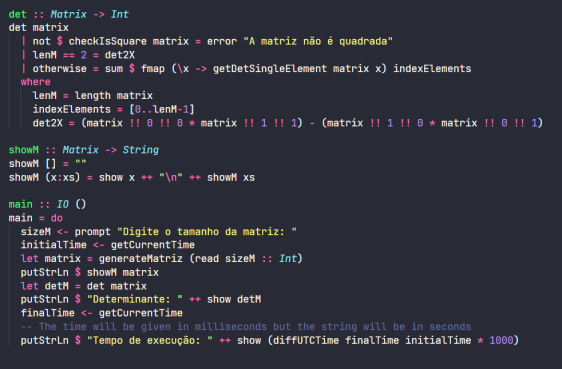
\includegraphics[scale=0.5]{codigo2.png} \\
        {\footnotesize Fonte: Elaborada pelo autor.}
        \label{fig:my_label}
    \end{figure}

   

\newpage

\section{COMPARAÇÃO DE TEMPO DE EXECUÇÃO}
 \begin{figure}[!ht]
        \centering
        \caption{Comparação entre gráficos que mostram o tempo de execução em milissegundos gerados pelo Python e Haskell}
        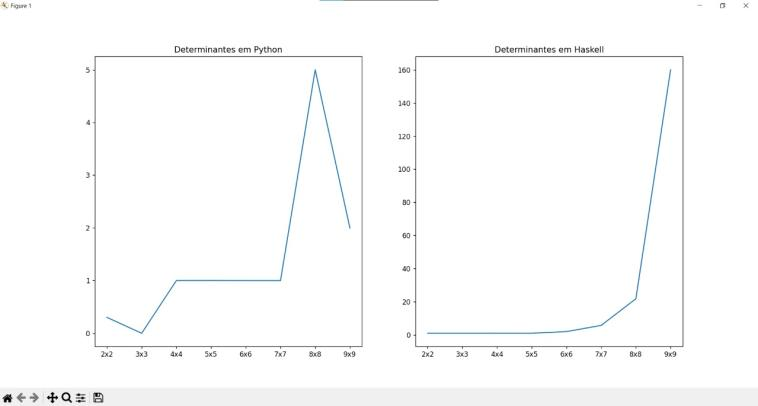
\includegraphics[scale=0.5]{comparacao_graficos.jpeg} \\
        {\footnotesize Fonte: Elaborada pelo autor.}
        \label{fig:my_label}
    \end{figure}

\section{REPOSITÓRIO DO PROJETO}
    \url{https://github.com/Anderson-Portes/haskell-matrix-determinant.git}
\end{document}
%